% !TeX spellcheck = it_IT
%Alberto Bobbo, Michele Bortone, Enrico Marcato
\documentclass[10pt, a4paper]{article}

\usepackage[scaled]{helvet}

\usepackage[utf8]{inputenc}
\usepackage[T1]{fontenc}
\usepackage[italian]{babel}

\usepackage{graphicx}
\usepackage{fix-cm}
\newcommand{\bigsize}{\fontsize{35pt}{20pt}\selectfont}
\newcommand{\mediumsize}{\fontsize{30pt}{20pt}\selectfont}
\newcommand{\normsize}{\fontsize{15pt}{10pt}\selectfont}


%crea uno spazio, utile perchè gli spazi extra dopo le macro
%vengono rimossi. Questo comando permette di inserirne uno.
\def\space{ }

\usepackage{float}
\usepackage{caption}

\usepackage{amsmath}
\usepackage{mathtools}

\usepackage{multirow}
%crea una cella per le tabelle in grado di andare a capo con \newline
%https://tex.stackexchange.com/questions/12703/how-to-create-fixed-width-table-columns-with-text-raggedright-centered-raggedlef
\usepackage{array}
\newcolumntype{L}[1]{>{\raggedright\let\newline\\\arraybackslash\hspace{0pt}}m{#1}}
\newcolumntype{C}[1]{>{\centering\let\newline\\\arraybackslash\hspace{0pt}}m{#1}}
\newcolumntype{R}[1]{>{\raggedleft\let\newline\\\arraybackslash\hspace{0pt}}m{#1}}

%puntini per l'indice
\usepackage{tocloft}
\renewcommand\cftsecleader{\cftdotfill{\cftdotsep}}


%https://tex.stackexchange.com/questions/4503/how-do-i-specify-color-in-rgb-using-hypersetup-in-hyperref
\usepackage{url}
\usepackage{ragged2e}
\usepackage{breakurl}
\usepackage[colorlinks=true]{hyperref}
\usepackage[hyperref]{xcolor}
\definecolor{UniPD}{RGB}{155, 0, 20}
\definecolor{Crema}{RGB}{220, 197, 149}
\definecolor{LinkNormNoClick}{RGB}{0, 0, 238}
\definecolor{LinkNormClick}{RGB}{69, 123, 157}
\hypersetup{colorlinks,breaklinks,
	urlcolor=UniPD,
	linkcolor=UniPD}

%per alcune liste
\usepackage{blindtext}
\usepackage{scrextend}
\addtokomafont{labelinglabel}
{\sffamily}


\newcommand{\Componenti}{Alberto Bobbo \newline Michele Bortone \newline
	Enrico Marcato}
\newcommand{\Referente}{Alberto Bobbo \newline alberto.bobbo@studenti.math.unipd.it}
\newcommand{\Gruppo}{Bobbo, Bortone, Marcato}
\newcommand{\Titolo}{Relazione Progetto Tecnologie Web}

\usepackage{lastpage} %info sul # dell'ultima pagina del documento
\usepackage{fancyhdr} %per modificare dimensioni,margini, intestazioni e righe a piè di pagina
\fancypagestyle{plain}{
	% cancella tutti i campi di intestazione e piè di pagina
	\fancyhf{}
	
	\lfoot{ %piè di pagina
		\Titolo{} \ - \textit{\Gruppo{}}
	}
	\rfoot{Pagina \thepage{} di \pageref{LastPage}} %es: pag: 4 di 10
	
	%linea orizzontale alle posizioni top e bottom della pagina
	\renewcommand{\headrulewidth}{0pt}  
	\renewcommand{\footrulewidth}{0.3pt}
}
\pagestyle{plain}

\usepackage{listings}


\lstdefinelanguage{HTML5}{
	sensitive=true,
	keywords={
		%% JavaScript
		typeof, new, true, false, catch, function, return, null, catch, switch, var, if, in, while, do, else, case, break, foreach, as,
		%% HTML
		html, meta, style, head, body, script, canvas, h1, h2, h3, h4, h5, h6, table, thead, tbody, tfoot, p, a, div, input, form, tr, th, label, ?php, ?, 
		%% CSS
		border:, transform:, -moz-transform:, transition-duration:, transition-property:,
		transition-timing-function:
	},
	% http://texblog.org/tag/otherkeywords/
	keywords=[2]{<, >, \, /, />, </ },  %%tag
	keywords=[3]{href, title, label, aria-label, lang, for, tabindex, placeholder, id, type, value, class, scope, }, %%attributi
	ndkeywords={class, export, boolean, throw, implements, import, this},
	keywords=[4]{echo, print\_ordinable\_th, REQUIRED},
	comment=[l]{//},
	% morecomment=[s][keywordstyle]{<}{>},  
	morecomment=[s]{/*}{*/},
	morecomment=[s]{<!}{>},
	morestring=[b]',
	morestring=[b]",    
	alsoletter={-},
	alsodigit={:}
}

\lstset{
	backgroundcolor=\color{background},
	tabsize=4,    
	language=HTML5,
	basicstyle=\ttfamily\linespread{1.15}\footnotesize,
	upquote=true,
	aboveskip={1.5},
	columns=fixed,
	showstringspaces=false,
	extendedchars=true,
	inputencoding=utf8,
	breaklines=true,
	prebreak = \raisebox{0ex}[0ex][0ex]{\ensuremath{\hookleftarrow}},
	frame=none,
	numbers=left,
	numbersep=5pt,	
	showtabs=false,
	showspaces=false,
	showstringspaces=false,
	basicstyle=\tiny\color{normal},
	identifierstyle=\color{normal},
	keywordstyle=\color{purple},
	keywordstyle=[2]\color{normal},
	keywordstyle=[3]\color{identifier},
	keywordstyle=[4]\color{blue},
	commentstyle=\color{comment},
	stringstyle=\color{string},
	numberstyle=\tiny\color{background}.
}



\begin{document}


\begin{titlepage}
\centering


\includegraphics[width=50mm]{Images/logo.png}
\vspace*{30px}
{\Large \\ \textbf{RELAZIONE PROGETTO TECNOLOGIE WEB}\\}
\vspace*{30px}

\bgroup
\def\arraystretch{1.3}
\centering

\begin{tabular}{c|L{5cm}}
\multicolumn{2}{c}{} \\ 
  \textbf{Componenti} & \Componenti{} \\
  \textbf{Referente} & \Referente{}
\end{tabular}
\egroup



\vspace*{80px}


\hypersetup{hidelinks}
\bgroup
\def\arraystretch{1.3}
\centering
\begin{tabular}{c}
\multicolumn{1}{c}{\textbf{Indirizzo Web Del Sito} } \\
  \url{http://tecweb2016.studenti.math.unipd.it/abobbo/pages/home.php}
\end{tabular}
\egroup

\vspace*{80px}

\begin{tabular}{c|L{4cm}}
\multicolumn{2}{c}{\textbf{Credenziali Admin} } \\ \hline
  \textbf{Username} & admin@progetto.com \\
  \textbf{Password} & admin
\end{tabular}
\quad
\begin{tabular}{c|L{4cm}}
\multicolumn{2}{c}{\textbf{Credenziali Utente} } \\ \hline
 \textbf{Username} & gino@progetto.com \\
  \textbf{Password} & ciaog
\end{tabular}

\vspace*{10px}

\end{titlepage}


\newpage
\hypersetup{hidelinks}
\tableofcontents
\newpage
\section{Presentazione sito}
Il sito in questione ha lo scopo di presentare l'evento musicale "Home Festival". Qui l'utente può trovare tutte le informazioni di cui ha bisogno per assistere ai vari concerti che avranno luogo durante il festival: in particolare vengono descritti brevemente i gruppi che parteciperanno all'evento ed è inoltre presente un insieme di indicazioni per raggiungere il luogo della manifestazione con i principali mezzi di trasporto.
È anche possibile effettuare una registrazione, che permette all'utente di commentare le ultime news sugli artisti partecipanti al festival, pubblicate dagli amministratori. 
\section{Utenti destinatari}
Il sito è destinato a tutti gli utenti che intendono partecipare all’Home Festival o che comunque desiderano avere indicazioni riguardo all’evento.  
All’interno del footer sono inoltre presenti alcuni contatti, nel caso l’utente volesse ricevere informazioni aggiuntive, e i link alle pagine dei principali social network, dove vengono inseriti gli ultimi aggiornamenti riguardanti il festival.
\section{Tipi di utenti}
Le categorie di utenti che il sito mette a disposizione sono:
\newline \textbf{Amministratore: }è in grado di pubblicare gli articoli che verranno inseriti nella sezione News tramite un form presente nella pagina stessa. Può inoltre rimuovere i commenti pubblicati dagli utenti sui vari articoli e commentare a sua volta.
\newline \textbf{Utente: }rappresenta l'utilizzatore vero e proprio del sito. Può commentare gli articoli pubblicati nelle News dagli amministratori.
\section{Progettazione}
\subsection{Organizzazione del sito}
Il sito presenta una barra di navigazione globale che contiene le varie aree del portale (Home, News, LineUp, Biglietti, Come Arrivare, Orari, Login e Registrati) e una barra di ricerca, utile per l'individuazione di particolari informazioni all'interno dell'intero sito.
Il codice della barra di navigazione è contenuto nel file nav.php, che viene richiamato da tutte le pagine.
\begin{figure}[h!]
  \centering
  
\includegraphics[width=1\textwidth]{Images/navbar.png}
  \caption{Barra di navigazione globale e barra di ricerca}
  \label{fig:navbar}
\end{figure}
\newpage
\subsection{Aree del sito}
\textbf{Home: }è la homepage del sito. La pagina è generata dinamicamente dal file home.php e presenta un form che permette agli utenti di iscriversi alla newsletter, una sezione dove viene visualizzato l'ultimo articolo inserito dagli amministratori e un'immagine che elenca i vari artisti che partecipano al festival musicale.
\begin{figure}[h!]
  \centering
  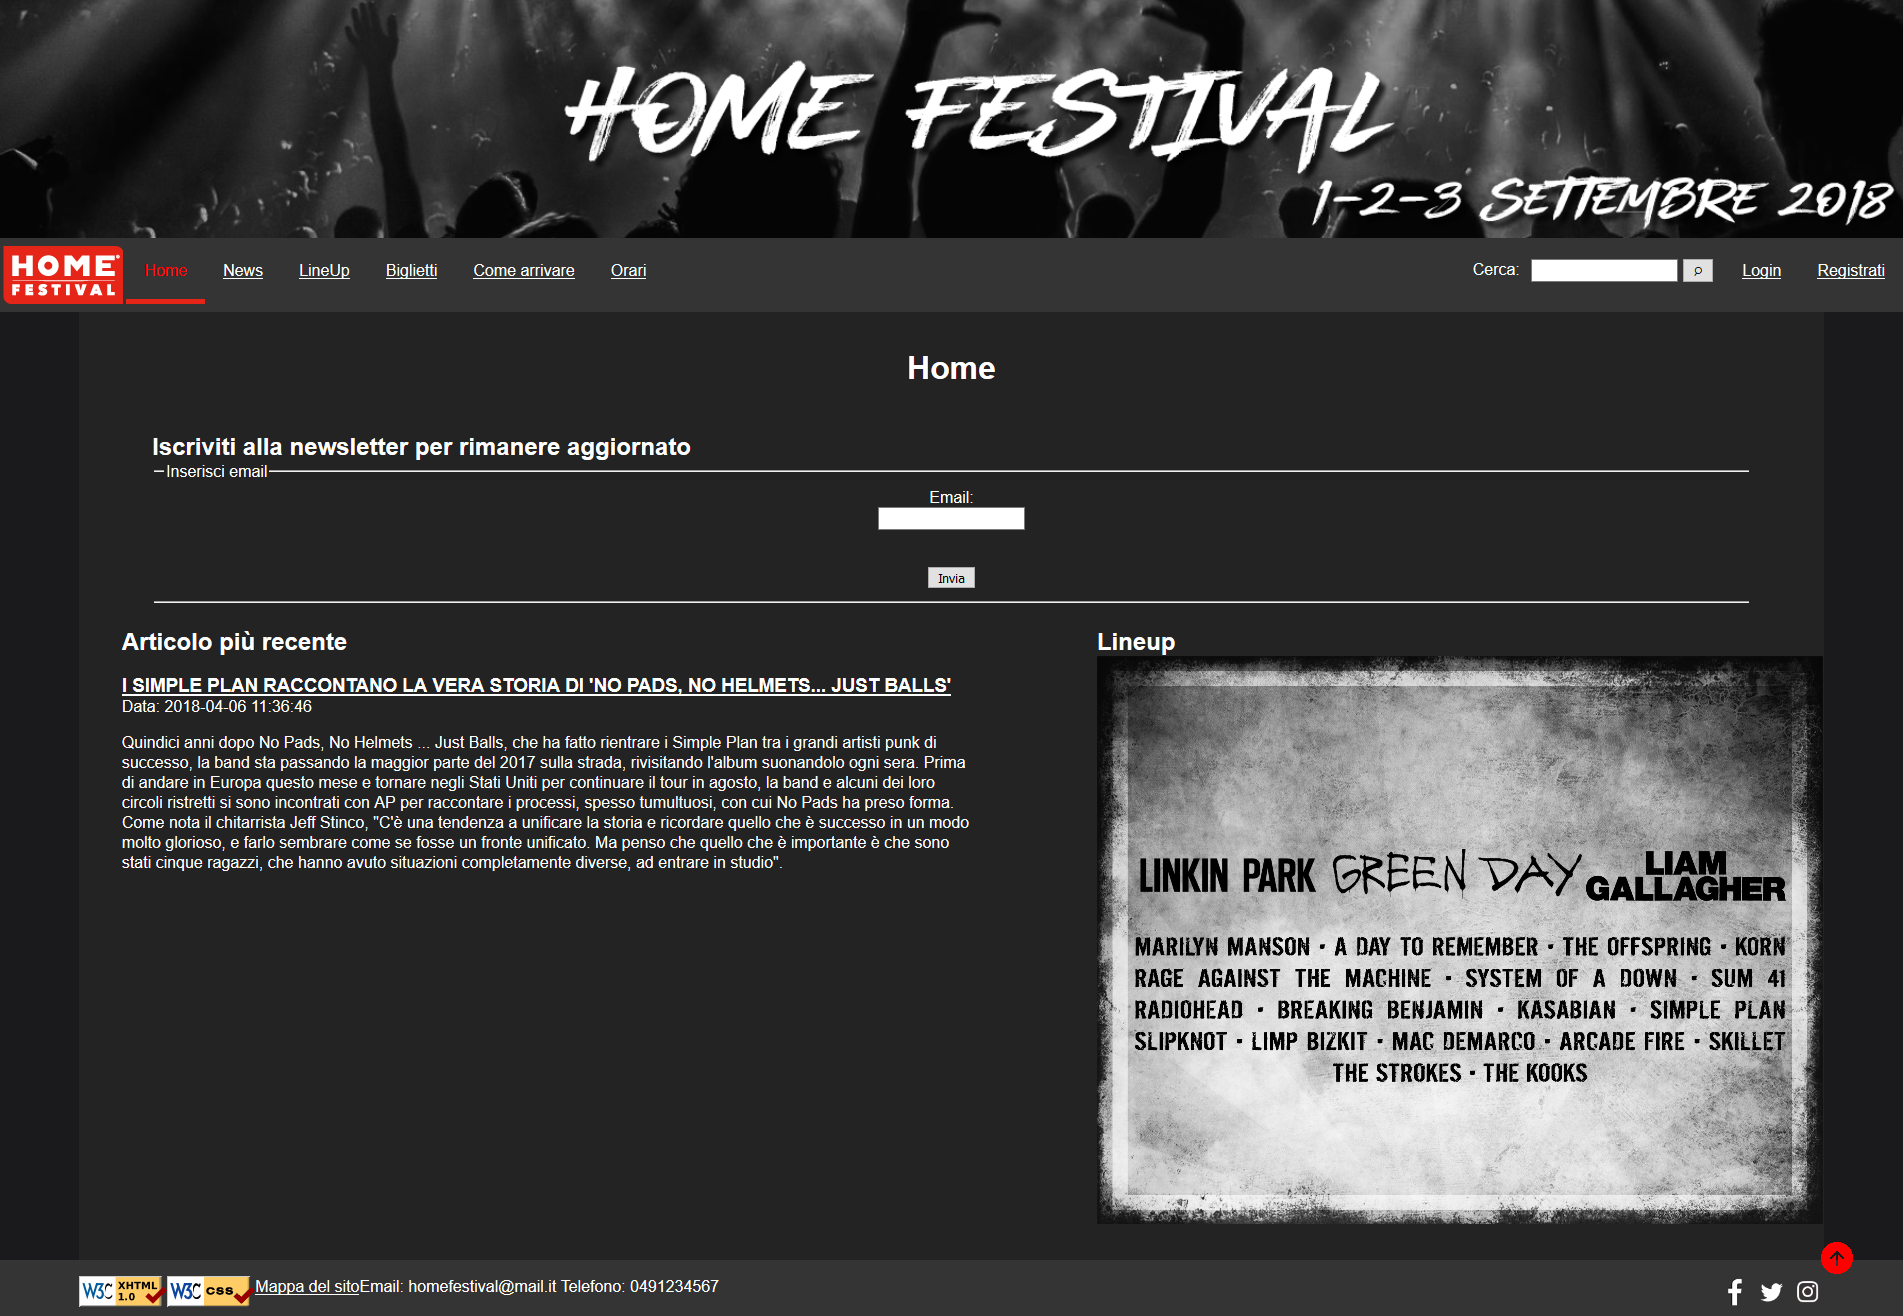
\includegraphics[width=1\textwidth]{Images/homepage.png}
  \caption{Homepage del sito}
  \label{fig:homepage}
\end{figure}
\begin{flushleft} \textbf{News: }contiene tutti gli articoli pubblicati sul sito. In ogni pagina sono visualizzati 5 articoli ed è possibile navigare tramite il menu di paginazione posizionato in coda alle news. L'utente può inoltre cliccare su un singolo articolo per visualizzarne la versione completa e, se ha anche effettuato il login, può scrivere un commento tramite il form apposito. La pagina viene generata dinamicamente dal file news.php, in modo da mantenere l'ordine cronologico degli articoli visualizzati. \end{flushleft}
\begin{figure}[h!]
  \centering
  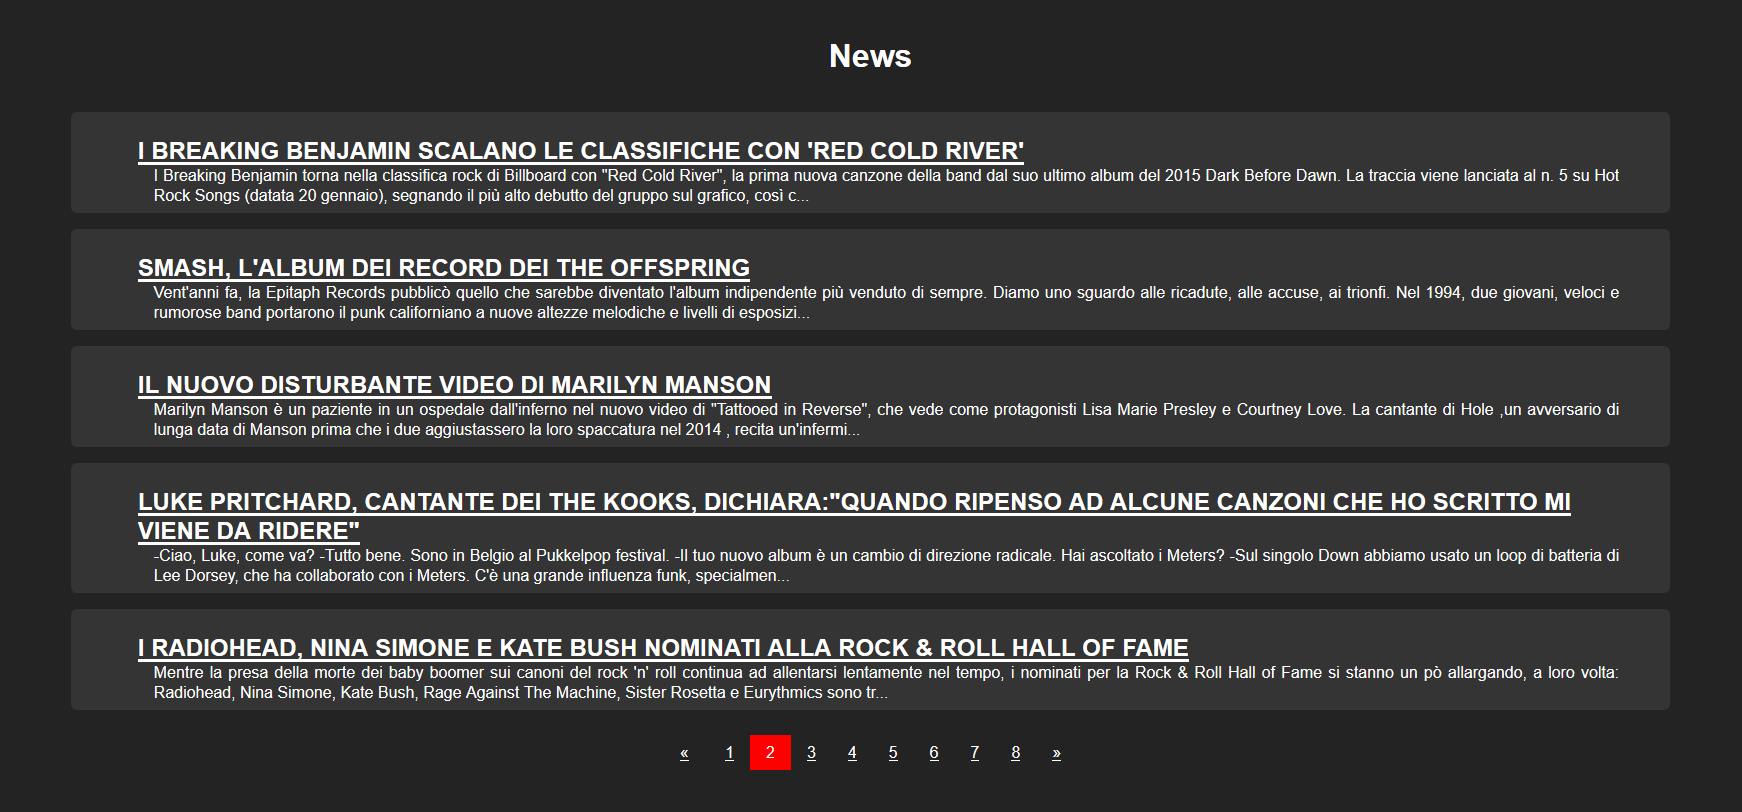
\includegraphics[width=1\textwidth]{Images/news.png}
  \caption{Pagina per la visualizzazione delle news}
  \label{fig:news}
\end{figure}
\begin{figure}[h!]
  \centering
  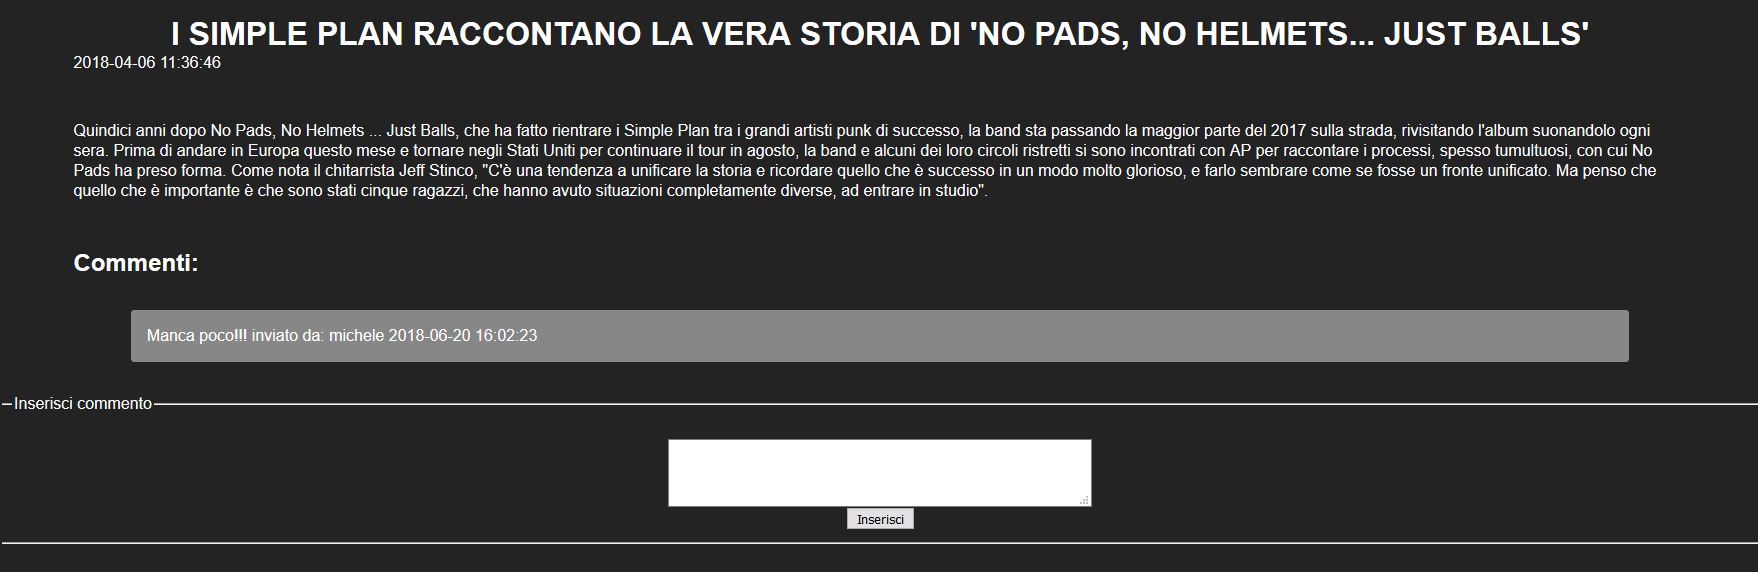
\includegraphics[width=1\textwidth]{Images/articolo.png}
  \caption{Pagina per la visualizzazione di un articolo con relativo form per l'inserimento di commenti}
  \label{fig:articolo}
\end{figure}
\newpage
\begin{flushleft} \textbf{LineUp: }presenta l'insieme degli artisti che partecipano all'evento, descritti da relative immagini e nomi. Cliccando sul nome del singolo artista è possibile accedere alla sua pagina dedicata, che contiene una breve descrizione della sua carriera e alcune informazioni generali. \end{flushleft}
\begin{figure}[h!]
  \centering
  \includegraphics[width=1\textwidth]{Images/lineup.png}
  \caption{Pagina che presenta tutti gli artisti che parteciperanno all'evento}
  \label{fig:lineup}
\end{figure}
\begin{figure}[h!]
  \centering
  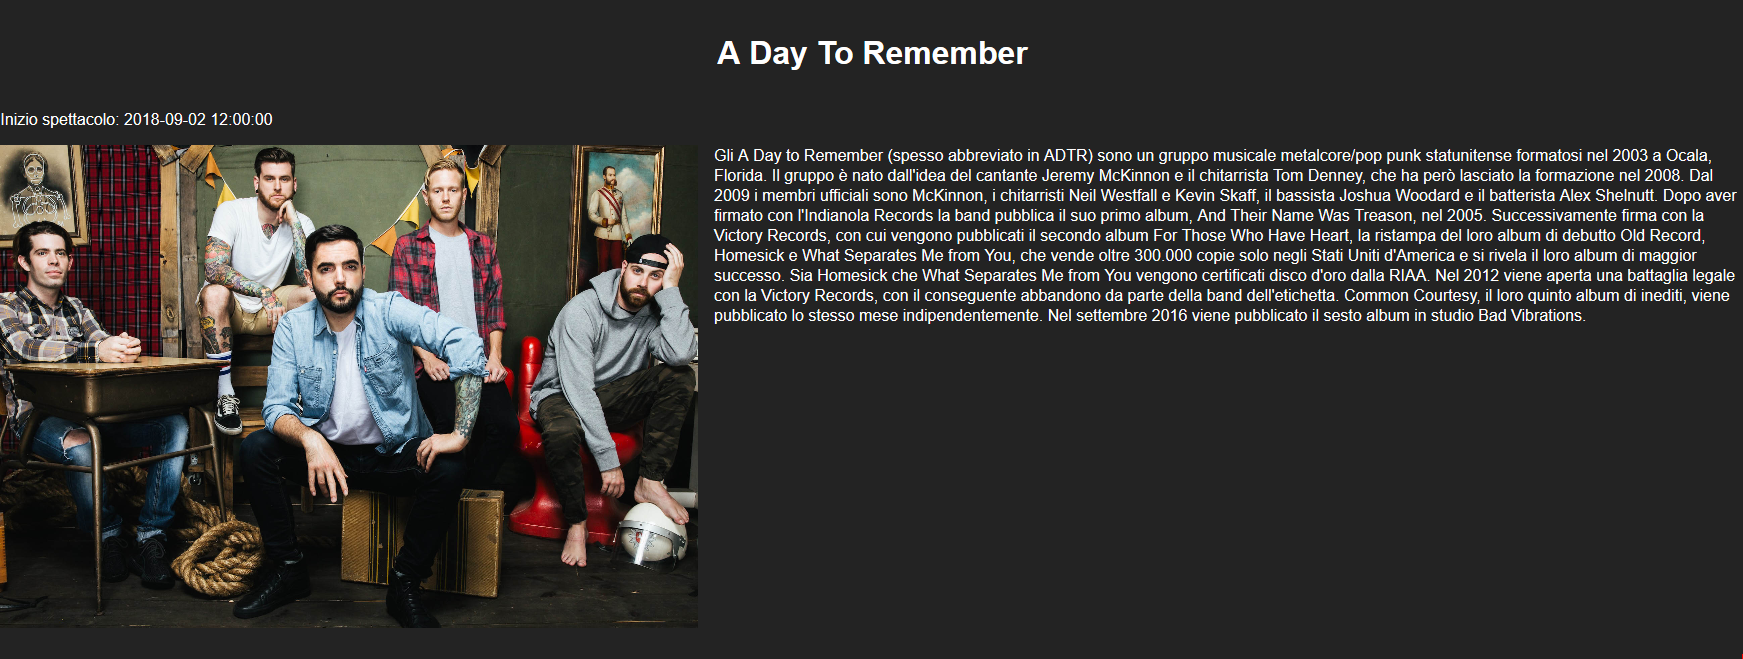
\includegraphics[width=1\textwidth]{Images/artista.png}
  \caption{Pagina che contiene le informazioni del singolo artista}
  \label{fig:artista}
\end{figure}

\newpage 
\vspace*{100px}
\begin{flushleft}\textbf{Biglietti: }fornisce all'utente le tipologie di biglietto che è possibile acquistare con una breve descrizione e il relativo prezzo.\end{flushleft}
\begin{figure}[h!]
  \centering
  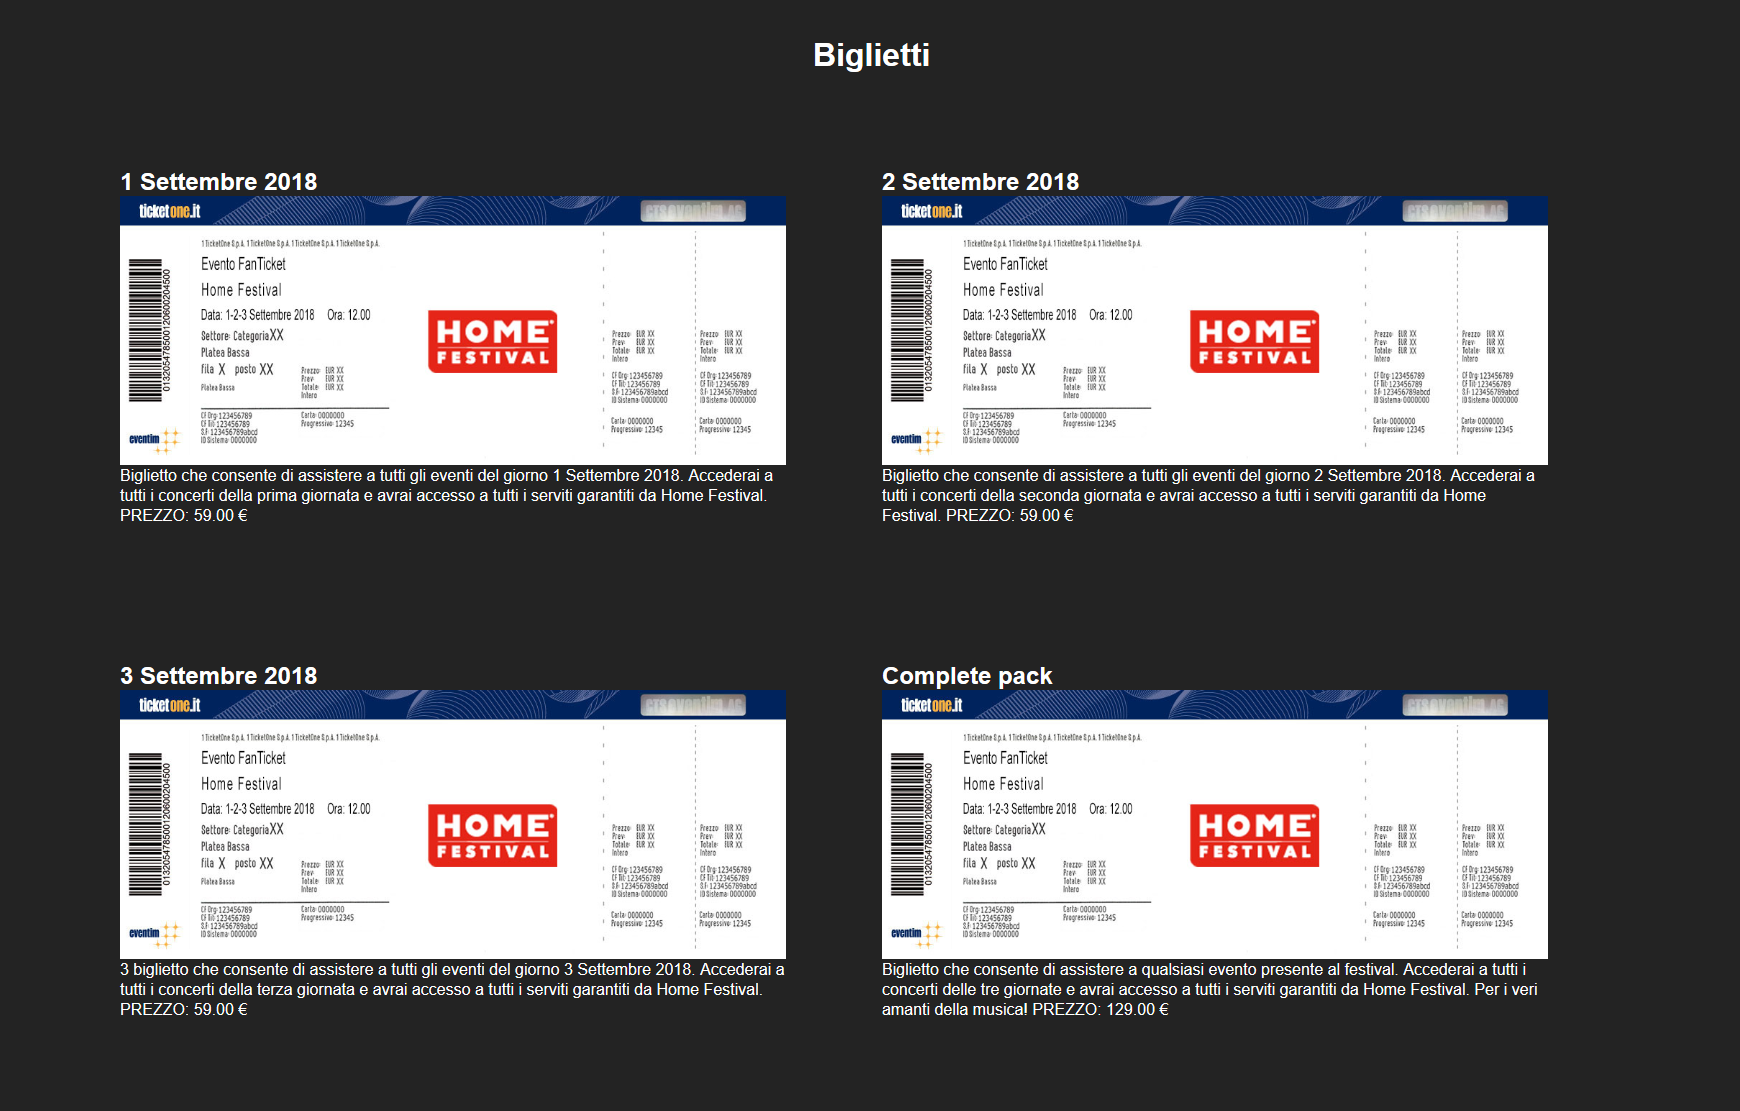
\includegraphics[width=1\textwidth]{Images/biglietti.png}
  \caption{Pagina con i vari tipi di biglietto disponibili per la partecipazione al festival}
  \label{fig:biglietti}
\end{figure}
\begin{flushleft} \textbf{Come Arrivare: }contiene una descrizione testuale delle indicazioni per raggiungere il luogo dell'evento con i principali mezzi di trasporto. Non è stata inserita una mappa per mantenere le informazioni della pagina il più accessibili possibile. \end{flushleft}
\begin{figure}[h!]
  \centering
 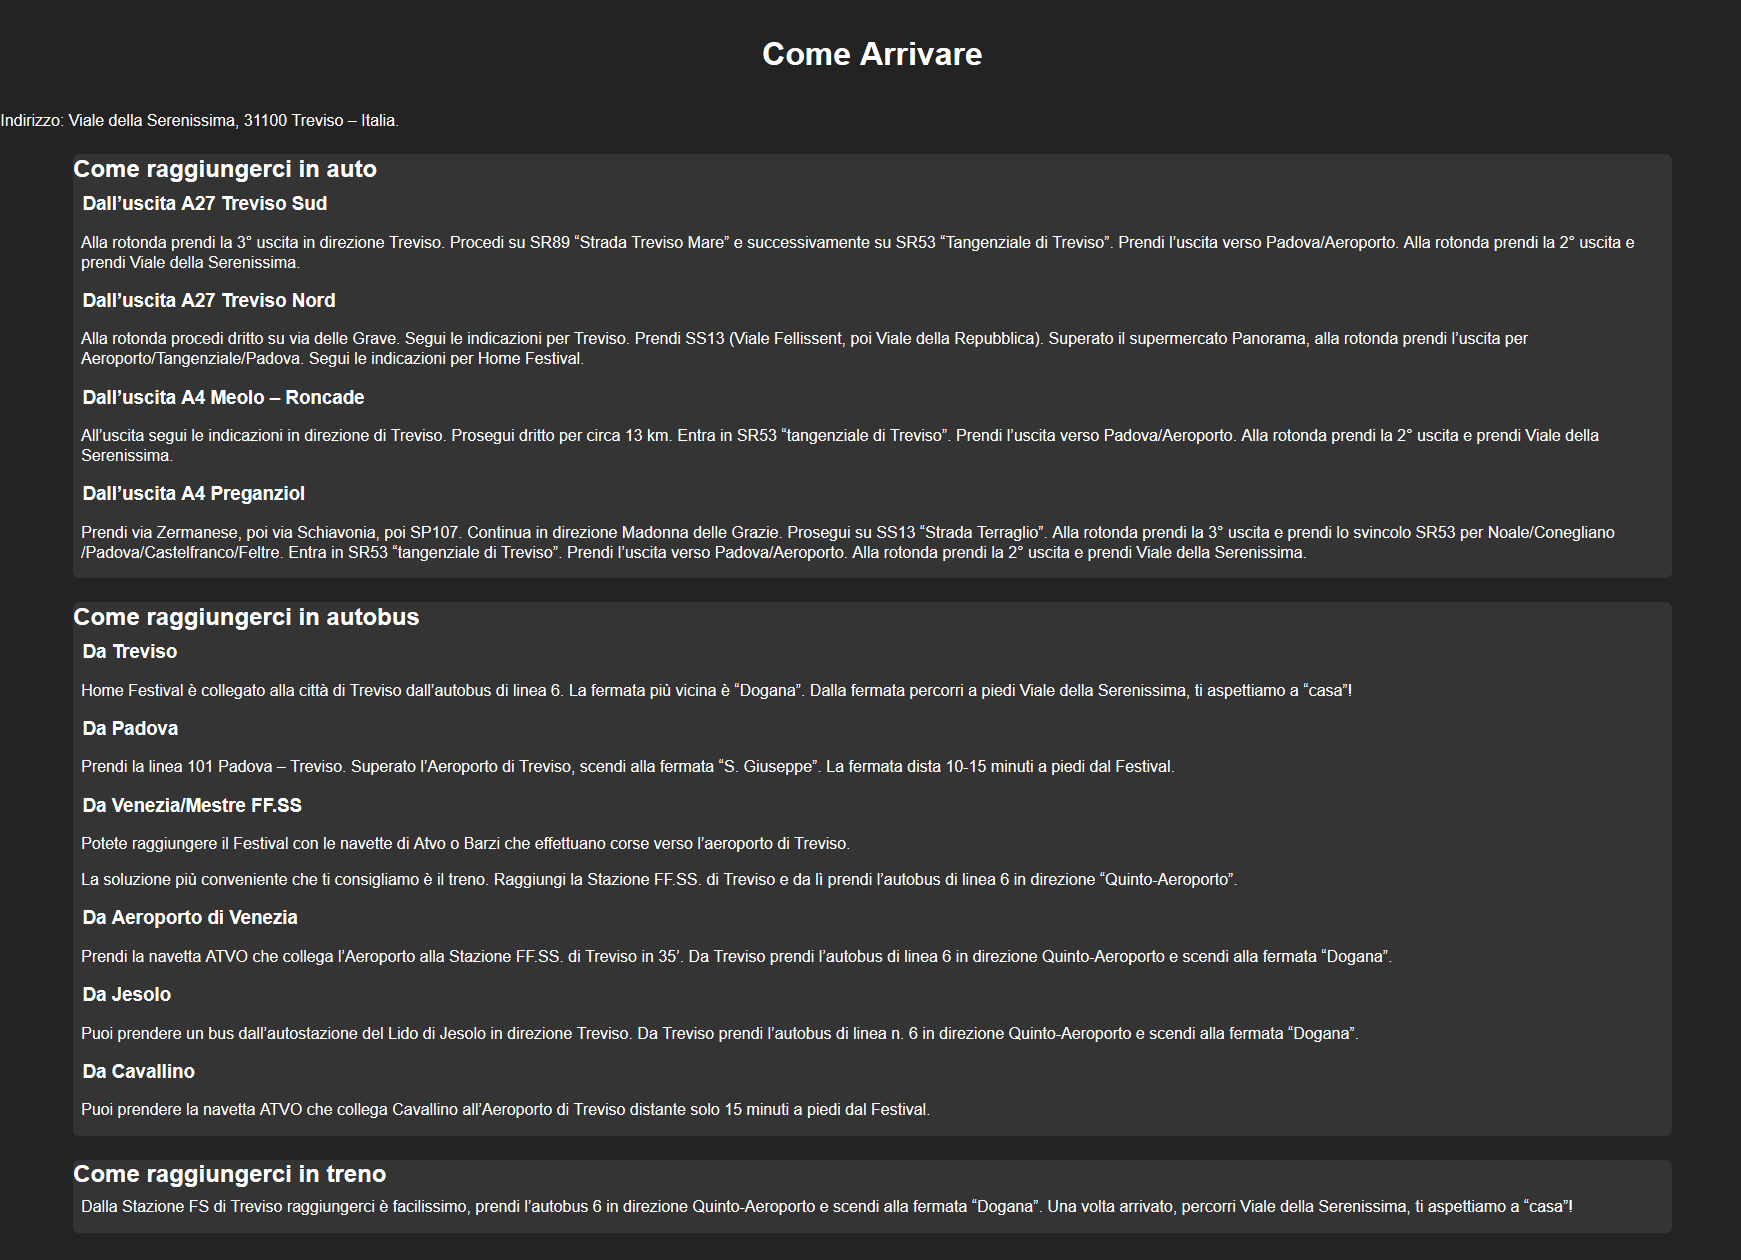
\includegraphics[width=1\textwidth]{Images/indicazioni.png}
  \caption{Indicazioni su come raggiungere il festival}
  \label{fig:indicazioni}
\end{figure}

\newpage

\begin{flushleft} \textbf{Orari: }presenta gli orari dei vari concerti che avranno luogo durante il festival, suddivisi per giornate. \end{flushleft}
\begin{figure}[h!]
 \centering
  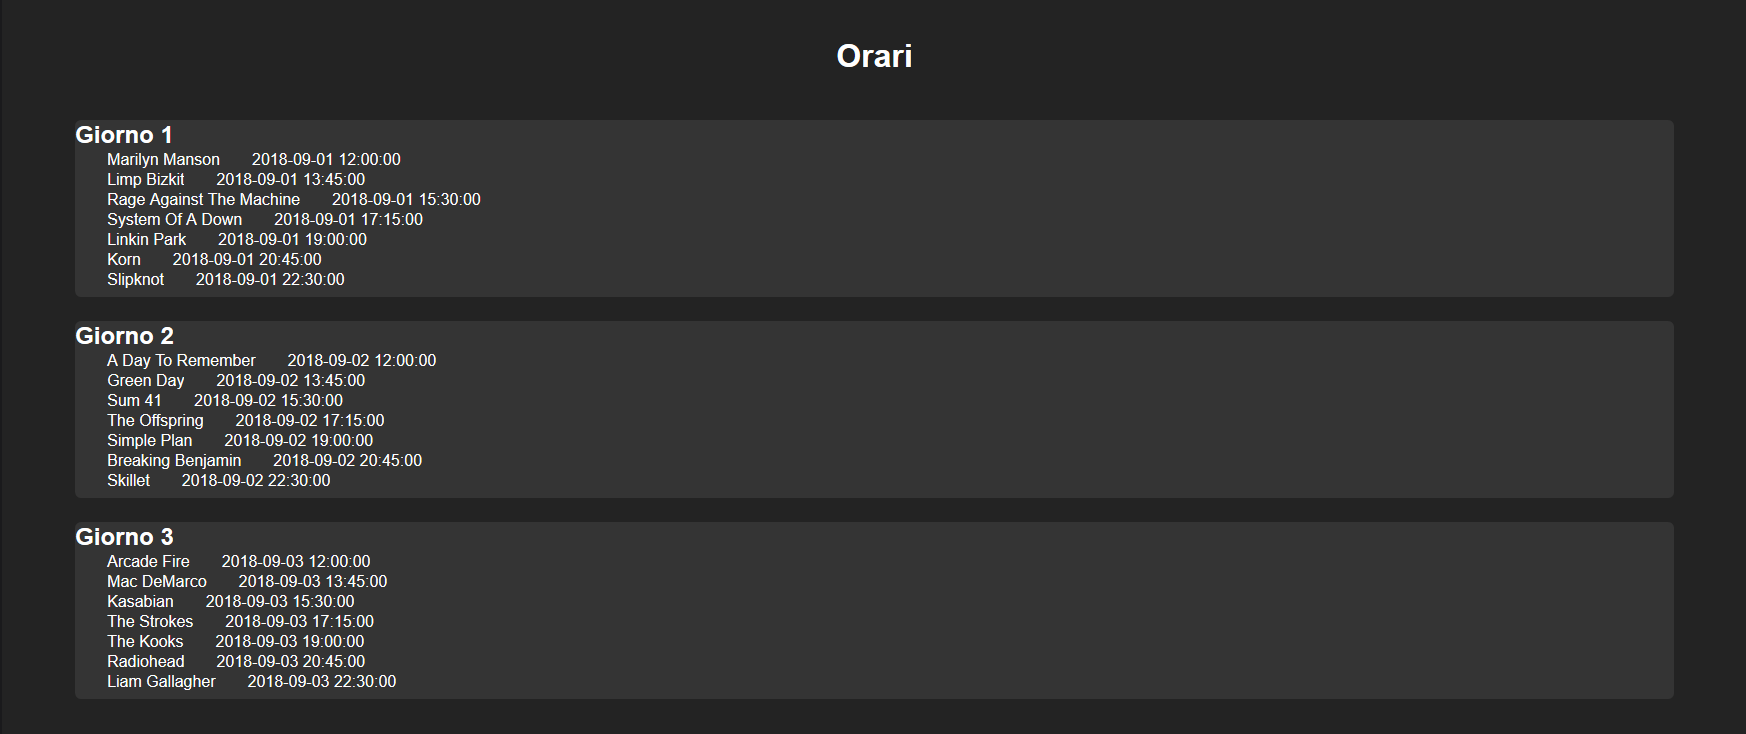
\includegraphics[width=1\textwidth]{Images/orari.png}
  \caption{Orari dei concerti che si tengono nelle 3 giornate del festival}
  \label{fig:orari}
\end{figure}

\begin{flushleft} \textbf{Login: }fornisce un form, sia agli utenti che agli amministratori, per effettuare il login al sito. Dopo aver completato l'accesso, l'utente può commentare gli articoli del sito, mentre gli amministratori possono anche eliminare i commenti e gli articoli inseriti. \end{flushleft}
\begin{figure}[h!]
 \centering
  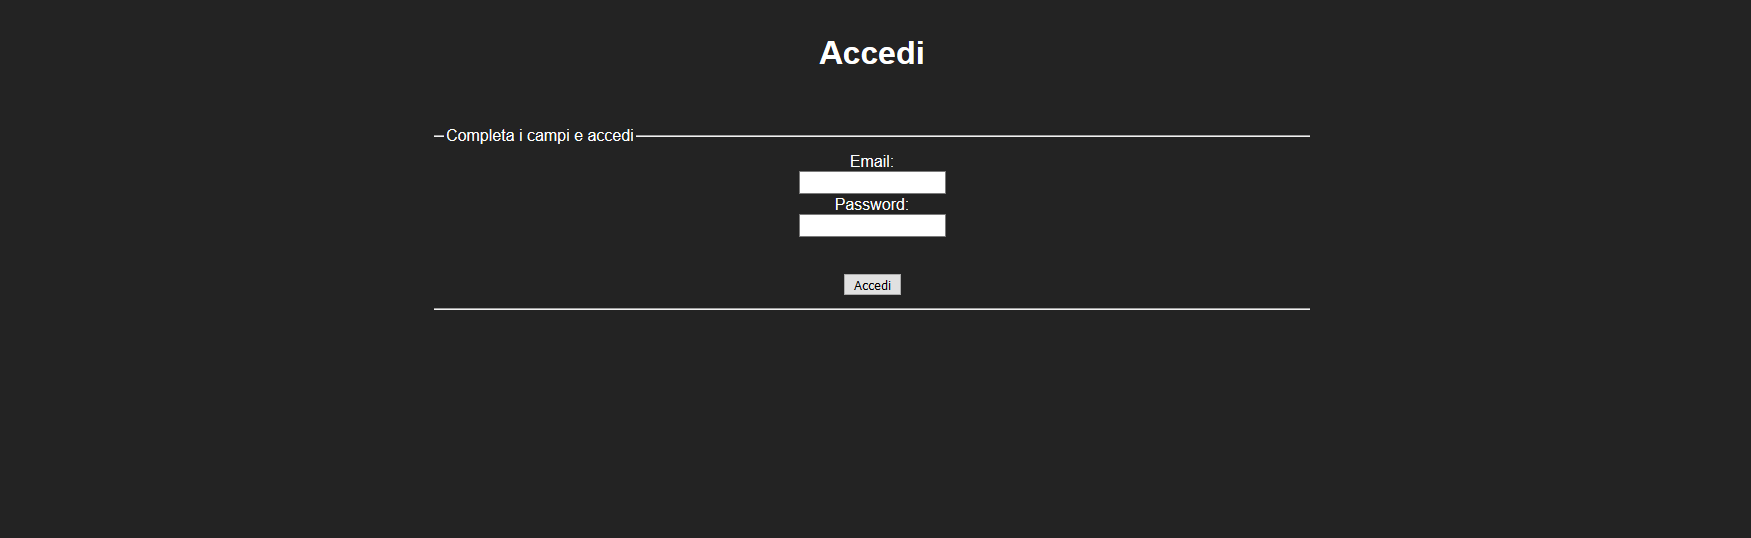
\includegraphics[width=1\textwidth]{Images/login.png}
  \caption{Pagina per effettuare l'accesso al sito}
  \label{fig:login}
\end{figure}
\begin{flushleft} \textbf{Registrati: }contiene un form che consente all'utente di effettuare la registrazione al sito inserendo i propri dati. Dopo che si è registrato, l'utente può accedere al sito con l'account che ha appena creato. \end{flushleft}
\begin{figure}[h!]
 \centering
  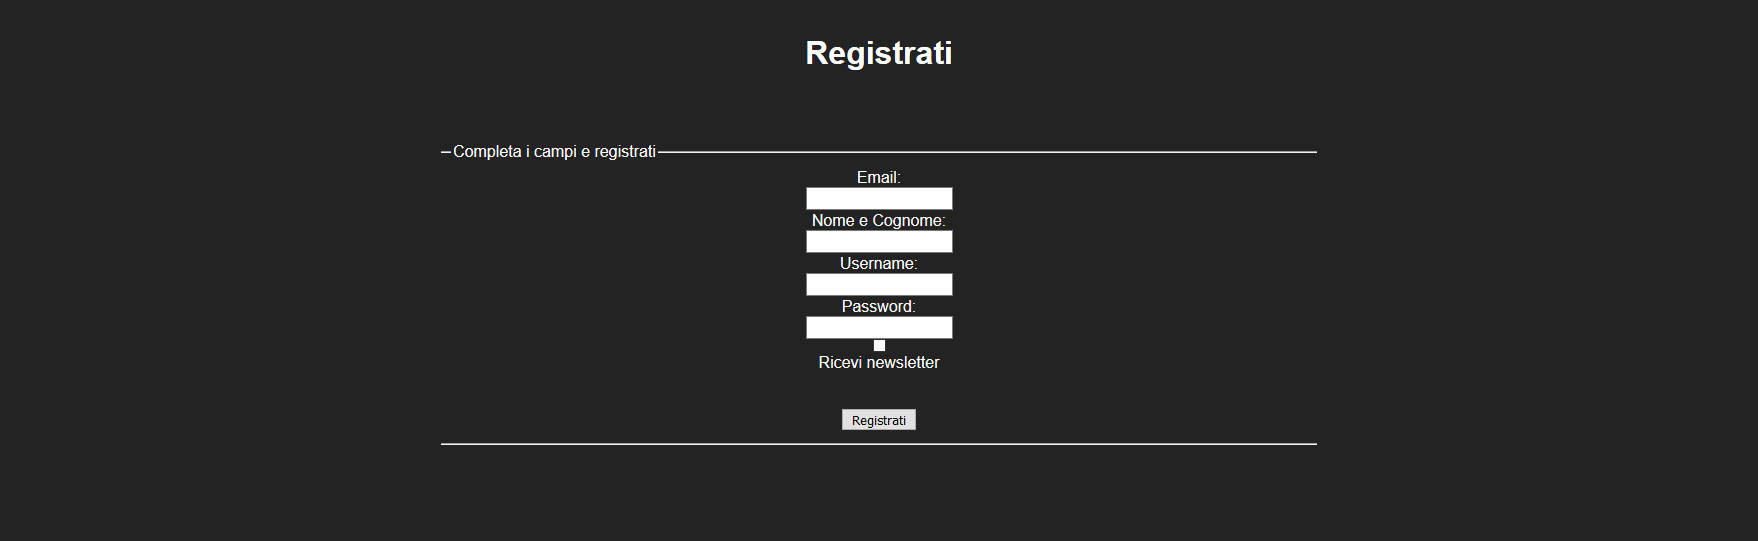
\includegraphics[width=1\textwidth]{Images/registrazione.png}
  \caption{Pagina contenente il form per la registrazione al sito}
  \label{fig:registrazione}
\end{figure}
\subsection{Struttura organizzativa}
Come struttura organizzativa è stato impiegato un database, dato che ogni elemento presente sul sito (utenti, articoli, commenti, artisti e biglietti), può essere ricondotto a un'entità all'interno della base di dati. Questo facilita la gestione e l'inserimento dei dati all'interno del sito.
\section{Accessibilità}
Per implementare un sito che fosse il più accessibile possibile, si è cercato di creare la massima separazione tra struttura, presentazione e contenuto. Inoltre, sono state seguite alcune linee guida presenti nel WCAG (Web Content Accessibility Guidelines), riportate di seguito, suddivise per categoria.

\subsection{Perceivable}

\subsubsection{Text Alternatives}
Tutti i contenuti non testuali presenti sul sito dispongono di un'alternativa testuale: le varie immagini inserite presentano tutte l'attributo \textbf{alt} nel caso venisse utilizzato uno screen reader per visitare il portale.

\subsubsection{Time-based Media}
I contenuti temporali all'interno di un sito risultano poco accessibili agli utenti con disabilità e per questo non sono stati inseriti.

\subsubsection{Adaptability}
Il sito può essere visualizzato su diversi dispositivi con dimensioni dello schermo differenti mantenendo sempre una struttura simile e non perdendo alcuna informazione. La versione per smartphone si differenzia dalle versioni desktop e tablet soprattutto per la navbar, la quale mantiene il logo del festival e la barra di ricerca, che hanno un'importanza prioritaria, mentre il menu per navigare all'interno sito viene sostituito da un unico bottone che, quando viene effettuato un tap, rende visibili le varie voci del menu. Per motivi di impaginazione, inoltre, negli smartphone non è presente l’immagine di testata.

\subsection{Understandable}

\subsubsection{Legibility}
Il testo inserito nel sito rimane sempre leggibile in quanto è stato utilizzato un colore per lo sfondo che ha un contrasto elevato con tutti gli elementi testuali presenti nelle varie pagine. Il sito è inoltre scritto con codifica UTF-8.


\subsubsection{Predictability}
Il sito rispetta i meccanismi di navigazione utilizzati nella maggior parte del web e presenta un aspetto uniforme in tutte le sue pagine interne per facilitare l'utente.


\subsubsection{Input Assistance}
Al momento della registrazione, dell’accesso al sito tramite credenziali e dell'iscrizione alla newsletter, i campi inseriti devono rispettare delle parametri per essere accettati dal server. L’utente, mentre esegue queste azioni, visualizza dei messaggi al di sotto dei textfield che lo aiutano attraverso la procedura.

\subsection{Robust}

\subsubsection{Compatibility}
Il sito è stato sviluppato utilizzando XHTML 1.0 e CSS 3.0 per favorire la compatibilità con il maggior numero di dispositivi e browser.

\subsection{Operable}

\subsubsection{Keyboard Accessibility}
È possibile navigare sul sito e compilare i vari form proposti utilizzando il tasto \textbf{TAB}. Le voci della navbar dispongono inoltre di access key, le quali facilitano la navigazione tramite screen reader.

\subsubsection{Time Availability}
Nel sito non sono stati inseriti contenuti temporizzati in quanto questi non risulterebbero usufruibili da tutti i visitatori del sito.

\subsubsection{Epilepsy}
Il sito non presenta contenuti che potrebbero creare problemi agli utenti affetti da epilessia.

\subsubsection{Navigability}
All'inizio di ogni pagina è stato inserito un link che rimanda direttamente al contenuto della stessa, trascurando la navbar e la barra di ricerca, in modo da facilitare la navigazione agli utenti non vedenti che utilizzano uno screen reader.

\subsection{Visione del sito da parte di individui con disturbi visivi}

Per simulare la visione del sito da parte degli utenti affetti da disturbi visivi, è stato utilizzato lo strumento fornito dall pagina http://www.color-blindness.com/coblis-color-blindness-simulator/. Di seguito vengono riportati i risultati ottenuti.

\subsubsection{Protanopia}

\begin{figure}[h!]
 \centering
  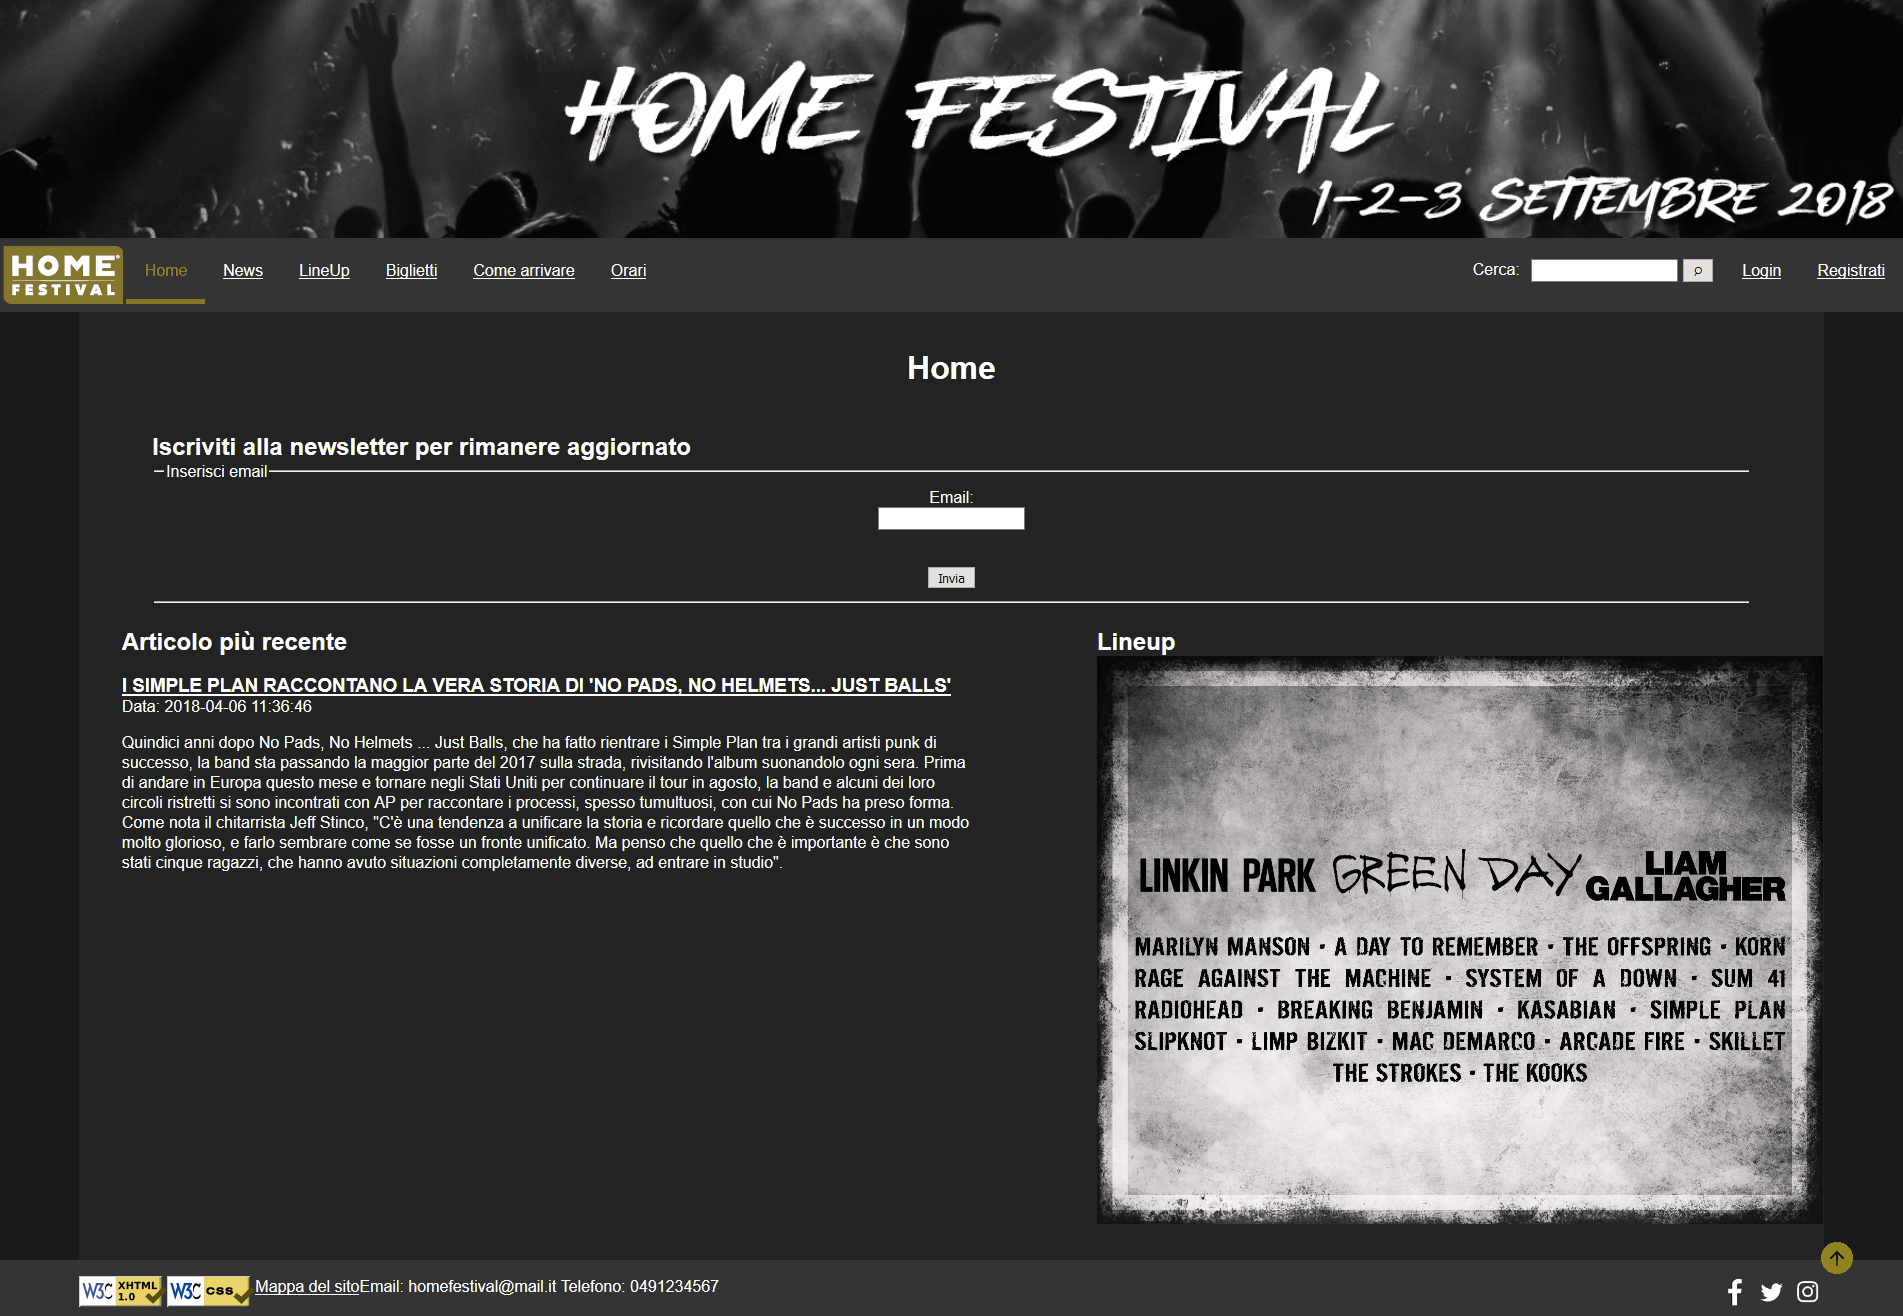
\includegraphics[width=1\textwidth]{Images/protanopia.png}
  \caption{Simulazione di protanopia}
  \label{fig:protanopia}
\end{figure}
\newpage
\subsubsection{Deuteranopia}

\begin{figure}[h!]
 \centering
  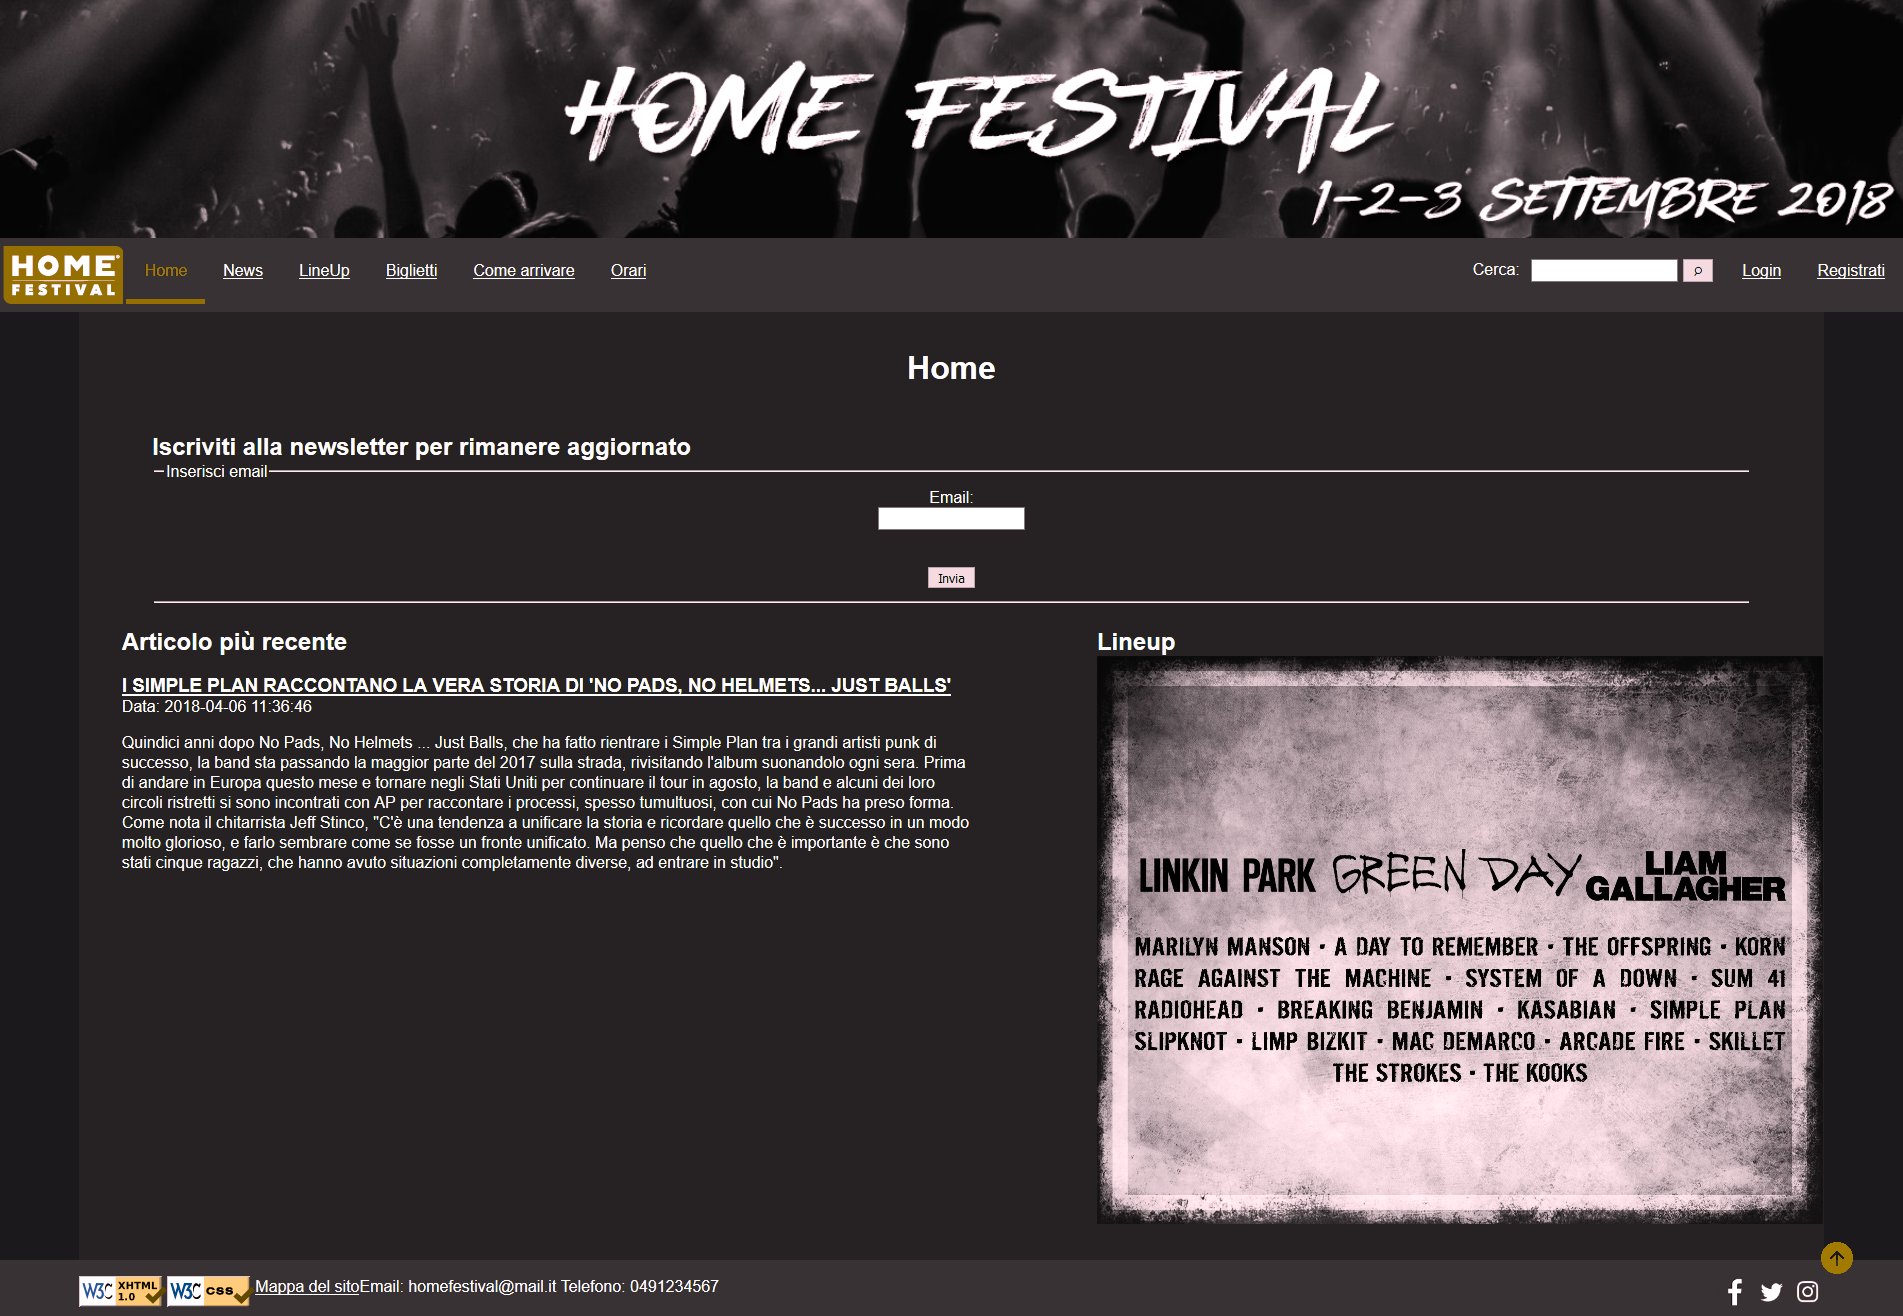
\includegraphics[width=1\textwidth]{Images/deuteranopia.png}
  \caption{Simulazione di deuteranopia}
  \label{fig:deuteranopia}
\end{figure}
\newpage
\subsubsection{Tritanopia}

\begin{figure}[h!]
 \centering
  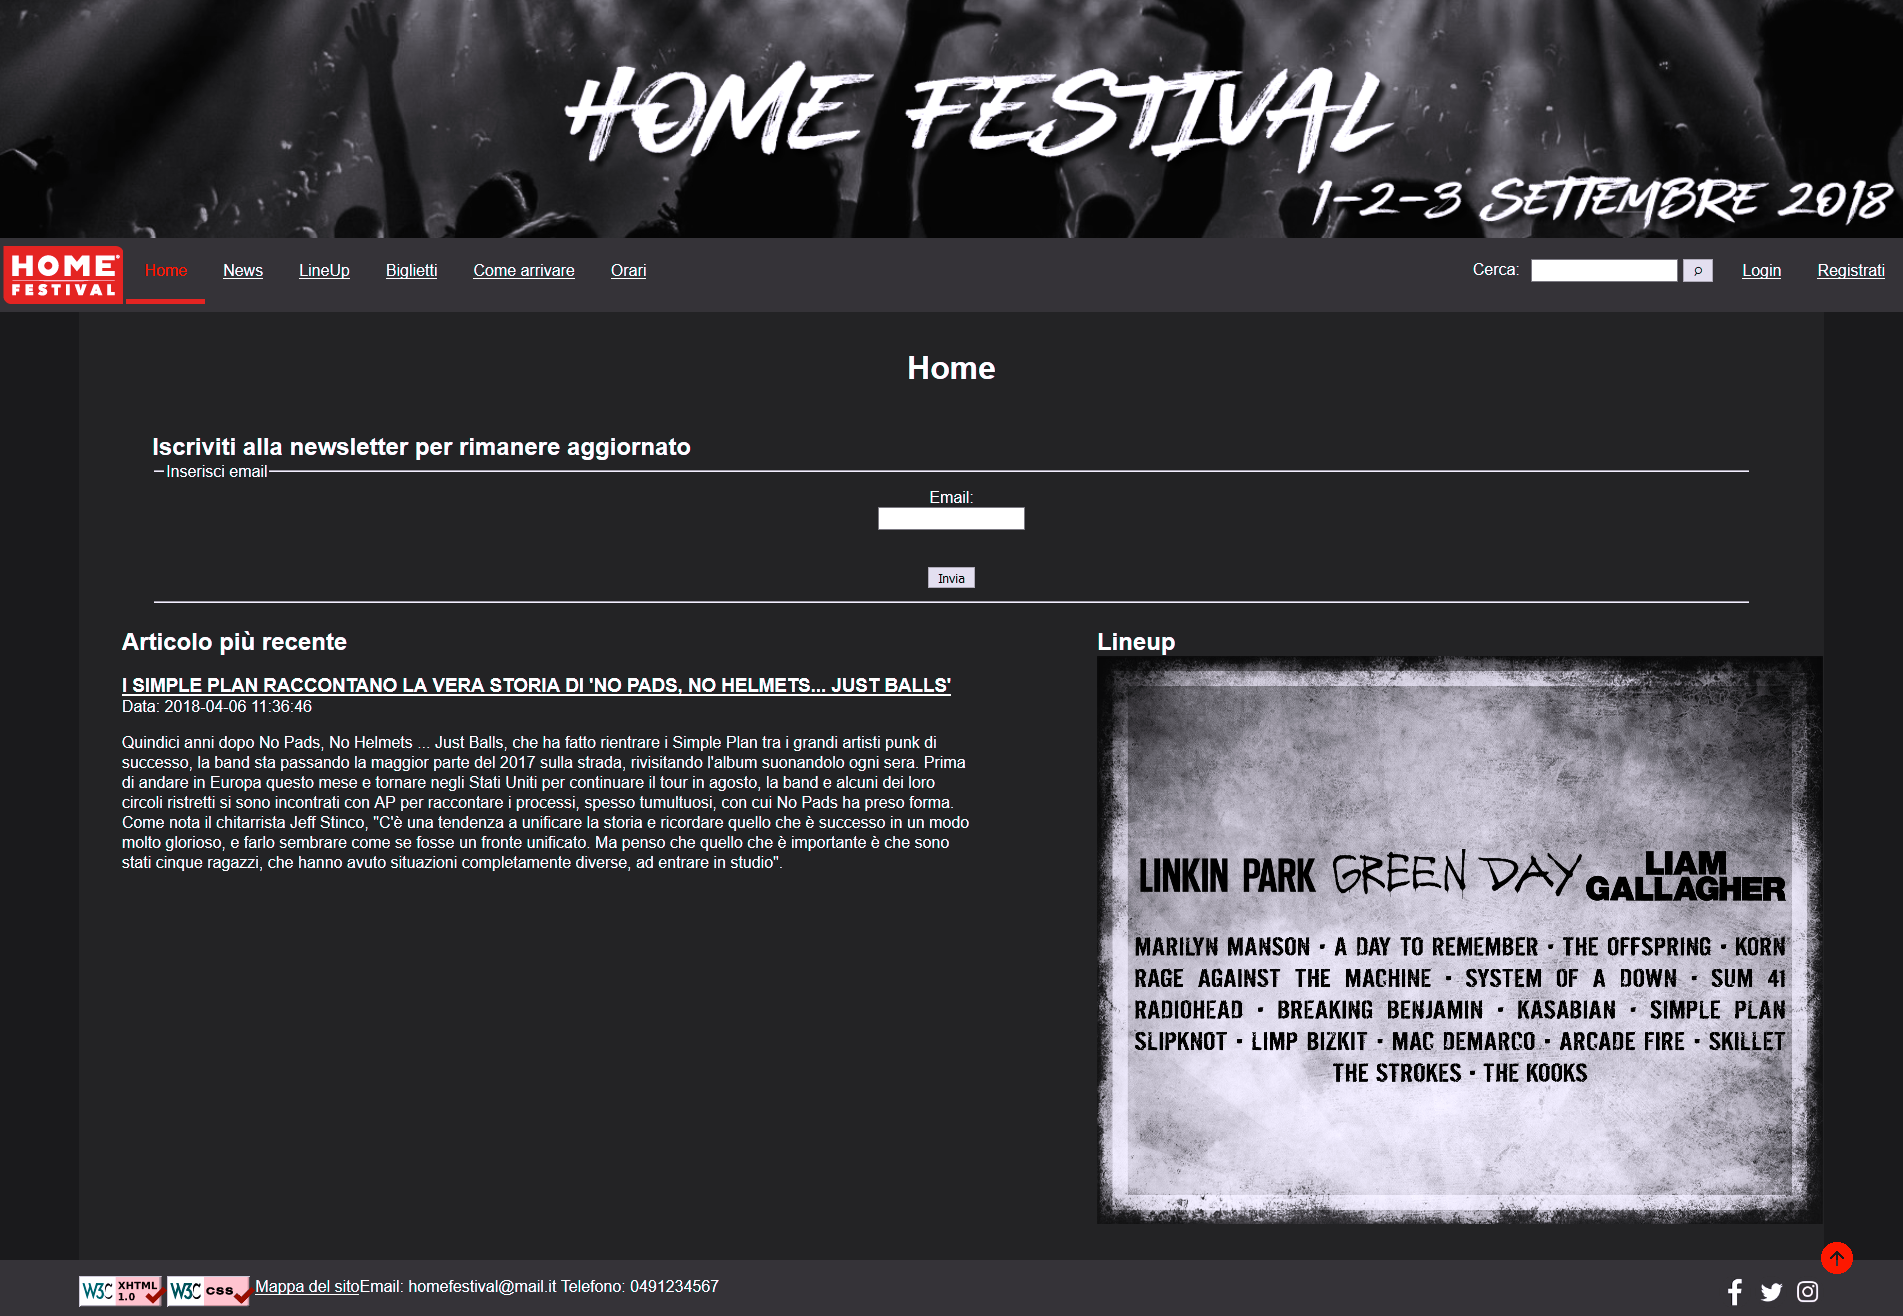
\includegraphics[width=1\textwidth]{Images/tritanopia.png}
  \caption{Simulazione di tritanopia}
  \label{fig:tritanopia}
\end{figure}

\subsection{Sintetizzatore vocale}
Per gli utenti non vedenti è stata prevista la navigazione all’interno del sito web, tramite l’utilizzo del tasto tab per scorrere i link della pagina, oppure degli access key personalizzati, in combinazione con un sintetizzatore vocale che ha lo scopo di leggere i link all’utente e di permettergli una comoda navigazione.
Durante lo sviluppo del sito sono stati effettuati dei test con il sintetizzatore vocale NVDA. Con l’uso di questo software open source, viene garantita una discreta navigabilità ed ogni volta che si preme il tasto tab viene letto il contenuto del link, si evidenzia se è già stato visitato e, qualora fosse presente, viene indicata la lettera corrispondente da premere per l’utilizzo degli access key. Una volta caricata la pagina con NVDA, viene selezionato, in automatico, un link invisibile, posizionato all'inizio della pagina, che permette all’utente non vedente di andare direttamente al contenuto saltando la navbar.

\section{Usabilità}


\subsection{Link}
Come si può notare nella Figura 1, tutti i link presenti nella barra di navigazione non sono circolari %%

\subsection{Navbar}
%%
\subsection{Motore di ricerca}
La decisione di inserire un motore di ricerca interno al sito è stata presa per dare la possibilità all’utente di ricercare un contenuto specifico nel modo più rapido possibile.
Ad esempio, è possibile inserire come parola chiave il nome di un artista e visualizzare nella pagina dei risultati tutti i contenuti a lui riferiti, la descrizione della sua carriera e i vari articoli correlati.
Per implementare questo motore di ricerca, sono state utilizzate delle query al database che ricercano le parole chiave all’interno del titolo o del testo di ogni news. La stessa ricerca viene effettuata anche nelle pagine di descrizione degli artisti.
La barra di ricerca è accessibile da ogni pagina, permettendo così all’utente di usufruirne in qualsiasi momento della navigazione.


\section{Amministratore, utente}

\subsection{Amministratore}

\subsection{Utente}

\section{Scelte Progettuali}
\begin{itemize}
	\item{Il form per l'inserimento di un articolo da parte dell'amministratore, che viene visualizzato se quest'ultimo ha effettuato il login, è posto al termine della pagina News, e non all'inizio, per favorire il controllo dell'articolo che è appena stato inserito}
	\item{Nella pagina orario non è stata utilizzata una tabella per formattare i dati in modo da evitare problemi di accessibilità}
	\item{Posizione form commento articolo...........................}
	\item{Link pagination non risultano visitati.....................................}
\end{itemize}

\section{Gerarchia dei file}
I file che compongono il sito sono contenuti nella cartella \textbf{public\textunderscore html} mentre le sessioni PHP sono salvate nella cartella \textbf{php\textunderscore sessions}. All'interno della cartella \textbf{public\textunderscore html} sono presenti il file index.html, utilizzato per effettuare il redirect a home.php, e alcune sotto cartelle indicate di seguito:
\begin{itemize}
  \item{\textbf{css}: contiene i file css utili alla presentazione del sito}
    \begin{itemize}
      \item{print.css: file css per la presentazione del sito su tutti i dispositivi}
      \item{style.css: file css per la stampa delle pagine}
    \end{itemize}
  \item{\textbf{images}: contiene}
    \begin{itemize}
       \item{Le immagini utilizzate nelle varie pagine del sito}
        \item{La cartella GroupsPic, dove sono presenti le immagini utilizzate nelle pagina LineUp}
    \end{itemize}
  \item{\textbf{js}: contiene il file javascript Script.js}
  \item{\textbf{layout}: contiene i file }
    \begin{itemize}
       \item{footer.php: file utilizzato da tutte le pagine per modellare il footer}
        \item{header.html: file utilizzato da tutte le pagine per modellare l'header}
        \item{nav.html: file utilizzato da tutte le pagine per modellare la barra di navigazione}
    \end{itemize}
  \item{\textbf{pages}: contiene i file PHP che compongono le pagine del sito}
\end{itemize}
\section{XHTML}
Per la progettazione del sito è stato utilizzato il linguaggio XHTML 1.0 con DTD Strict piuttosto che HTML 5, per ottenere una buona compatibilità su più dispositivi e browser possibile.
XHTML 1.0 Strict, a differenza della versione Transitional, non accetta i tag HTML definiti deprecati, non è tollerante alle non conformità sintattiche e prevede controlli più rigorosi anche rispetto al valore di alcuni attributi dei tag.

\section{PHP}
%%DA LEGGERE%%
Per produrre del codice XHTML dinamico si è scelto di utilizzare PHP che garantisce facilità nell’interazione con il database per il recupero dei dati visualizzati nelle pagine.
In quasi tutte le pagine infatti, è stato inserito del codice php che serve per accedere al database, recuperare specifici dati (in base alla tipologia della pagina), e stamparli a schermo  in codice XHTML.
Tutte le pagine che compongono il sito web hanno estensione .php ad eccezione di index.html che non fa altro che reindirizzare ad home.php (la pagina principale del sito web) e header.html che contiene l’immagine di testata con le date in cui si svolgerà il festival.
Le componenti comuni in ogni pagina, cioè come navbar e footer, sono state realizzate in file separati chiamati rispettivamente nav.php e footer.php che poi vengono richiamati nelle varie pagine.
Con questo tipo di approccio, nel caso si voglia successivamente sostituire gli elementi della pagina che sono comuni a tutte le pagine basterà modificare un solo file.
Php permette di usare sia uno stile procedurale che uno stile orientato agli oggetti. Principalmente per comodità d’uso, si è preferito utilizzare uno stile procedurale del codice dato che ogni pagina ha richiesto del codice PHP specifico per ogni funzionalità offerta.

\subsection{Descrizione file}
\textbf{article.php}
Il codice contenuto in questo file ha lo scopo di stampare a schermo l’articolo che l’utente vuole visualizzare. Per fare ciò, recupera i dati dal database tramite una serie di query che selezionano l’articolo corretto da visualizzare e i commenti correlati.
Inoltre nel caso sia loggato un utente compare anche un form per l’inserimento di un commento all’articolo e un link che dà la possibilità di eliminare i propri commenti.
Se l‘utente loggato è un amministratore, può eliminare qualsiasi commento, anche di altri utenti, oppure l’articolo stesso. 
Sono stati implementati anche dei controlli sull’inserimento dei commenti che non permettono la pubblicazione di un commento vuoto, infatti in caso di errore l’utente verrà avvisato tramite un messaggio di errore e il commento non sarà salvato nel database.


\textbf{artista.php}
Grazie all’interrogazione del database, questo file restituisce all’utente la pagina di descrizione di un artista.
Viene mostrato a schermo nome, orario dello spettacolo, un’immagine dell’artista ed una breve descrizione. 


\textbf{biglietti.php}
Tramite query, recupera dal database le informazioni sulle tipologie di biglietto disponibili.

\textbf{connection.php}
Questo file contiene le righe di codice php che permettono di stabilire una connessione al database.
Viene richiamato quando si necessita di interrogarlo.

\textbf{footer.php}
Contiene tutti i contatti comprese le icone di vari social network e un link alla mappa del sito.
Inoltre sono stati inseriti anche i loghi del W3C che certificano la validazione del codice XHTML e CSS.
Questo file viene richiamato in ogni pagina del sito e si occupa anche di chiudere la connessione al database.


\textbf{home.php}
Genera la home del sito. La funzionalità principale è quella di iscrizione alla newsletter, infatti inserendo la propria email (senza la l’obbligo di creare un vero e proprio account), si potrà ricevere aggiornamenti sugli articoli e le varie novità del festival.
Inoltre viene mostrato a schermo l’articolo più recente e l’immagine della lineup che, se cliccata, rimanda alla pagina dedicata

\textbf{lineup.php}
Sempre tramite interrogazioni al database, viene generata una griglia contenente tutti gli artisti presenti al festival. Per ogni artista è presente un’immagine che lo rappresenta e un link per visualizzare la pagina di descrizione del singolo artista.
 
\textbf{login.php}
Contiene il form per accedere al proprio account. Nel caso che i dati inseriti siano sbagliato verrà mostrato un messaggio che segnale all’utente l’errore dei dati nell’ inserimento, mentre se i dati sono stati inseriti correttamente si verrà reindirizzati alla home.

\textbf{logout.php}
Chiude la sessione e reindirizza alla pagina di login.

\textbf{map.php}
Pagina statica contenente l’indirizzo del luogo in cui si svolge il festival e le informazione su come arrivarci. Php viene utilizzato solo per richiamare i file che generano la navbar e il footer.

\textbf{mapsite.php}
Altra pagina statica contenente tutti i link per navigare all’interno del sito ed una loro breve descrizione. Questa pagina è accessibile dal footer.

\textbf{nav.php}
Grazie al richiamo di questo file viene generata in ogni pagina la navbar dalla quale si può accedere a tutte le categorie principali del sito.
Al suo interno è presente anche una barra di ricerca per poter accedere in maniera rapida a contenuti specifici ricercati dall’utente.
La navbar viene generata dinamicamente e cambia a seconda della pagina visualizzata dall’utente in modo da evitare link circolari e permettere all’utilizzatore di aver sempre chiaro dove si trova all’interno del sito.

\textbf{news.php}
Questo file genera la pagina delle news che è composta da un’anteprima di 5 articoli ordinati cronologicamente.
È stata implementata una paginazione degli articoli in stile motore di ricerca. Questa parte di codice calcola il numero effettivo degli articoli presenti nel database e li stampa di 5 in 5 in base al numero della pagina selezionata.
Se si è loggati come utente amministratore, compare anche un form, con relativi controlli di inserimento dati ed eventuale messaggio di errore, che permette agli admin del sito di inserire un nuovo articolo nel database.


\textbf{orari.php}
Questo file non fa altro che interrogare il database per stampare a schermo gli orari di esibizione dei vari artisti nei tre giorni di festival. 

\textbf{register.php}
File che si occupa della registrazione di un nuovo utente.
È previsto un form per l’inserimento dei dati personali e la possibilità tramite una checkbox di registrarsi contemporaneamente anche alla newsletter. In fase di registrazione i controlli sono molto rigidi e qualora i dati non siano corretti, verrà mostrato a schermo un messaggio di errore specifico per la casella di testo contenente il dato errato e anche nel caso in cui l’email sia già stata utilizzata.

\textbf{search.php}
In questa pagina vengono mostrati i contenuti richiesti dall’utente tramite il piccolo motore di ricerca implementato nel sito.
I risultati possono essere di due tipi: l’anteprima della pagina di un artista oppure l’anteprima di un articolo.
Le anteprime sono cliccabili e portano direttamente al contenuto completo.


\section{Javascript}
Il linguaggio Javascript è stato utilizzato per aiutare l’utente nell'inserimento dei dati all'interno delle pagine di login, registrazione e home. Se il campo è stato compilato correttamente, compare un messaggio verde di conferma, altrimenti uno di errore, di colore rosso. L’email deve contenere obbligatoriamente i caratteri ‘@’ e ‘.’;  la password e l'username devono essere di almeno 4 caratteri; nome e cognome, che vanno inseriti in un unico campo, devono essere separati da uno spazio. Se un utente non ha attivato Javascript nel browser, è possibile disporre comunque di ogni funzionalità del sito, esclusi i messaggi di conferma ed errore. Nel caso in cui i dati errati vengano inviati al server, verranno eseguiti tramite codice PHP, gli stessi controlli precedentemente eseguiti in Javascript. La pagina dell’utente verrà ricaricata e sarà restituita la tipologia dell’errore.
È stato ritenuto non necessario inserire dei controlli in Javascript per l'inserimento di commenti riguardanti gli articoli, in quanto si presuppone che l’utente non inserisca commenti vuoti. Nel caso dovesse accadere, un controllo lato server, realizzato in PHP, ne impedirà l’inserimento. Solo gli amministratori dispongono dei permessi per inserire nuovi articoli. Nel caso venga erroneamente effettuato il submit di una news vuota, questo verrà interrotto dal lato server. 
Un’altra funzionalità implementata tramite Javascript è la possibilità di ritornare all'inizio della pagina cliccando sul bottone rosso, posto in basso a destra all'interno della schermata.

\section{Validazione}
Il sito è stato validato tramite W3Validator per quanto riguarda i linguaggi XHTML 1.0 e CSS 3.0; è possibile verificarlo nel footer, dove sono stati aggiunti i certificati di validazione. Per avere un’ulteriore conferma sulla validità del codice XHTML, si è fatto anche uso dell’applicazione TotalValidator. Vengono evidenziati 3 warnings:
\begin{itemize}
\item{Add a skip navigation link as the first link on the page}
\item{Different adjacent links that use the same link text may be confusing: See matching tag on line}
\item{Different adjacent links that use the same link text may be confusing: See matching tag on line}
\end{itemize}
Il primo warning è dato dal fatto che il validatore non riconosce il link posto in cima alla pagina, il quale permette agli utenti non vedenti di saltare al contenuto del sito, evitando la lettura del menù ogni qualvolta si giunge in una nuova pagina. 
Gli altri due warnings sono dovuti alla presenza di due link identici nella stessa pagina. In particolare, i due link, posti sottoforma di bottone, rimandano entrambi all'inizio della pagina, ma uno è visibile solo con Javascript attivo mentre l'altro, al contrario, appare quando questa condizione non si verifica. 


\section{Compatibilità browser}
Il: Internet Explorer, Microsoft Edfge, Opera, Safari, Chrome e Mozilla Firefox.
Per quanto riguarda i dispositivi mobili, il
\subsection{Compatibilità con Internet Explorer}

\subsubsection{Internet Explorer 8}
%%

\subsubsection{Internet Explorer 11}
%%

\subsection{Compatibilità con Microsoft Edge}
Il sito viene visualizzato correttamente e dispone di tutte le sue funzionalità.

\subsection{Compatibilità con Opera}
%%

\subsection{Compatibilità con Safari}
%%

\subsection{Compatibilità con Chrome}
Il sito viene visualizzato correttamente e dispone di tutte le sue funzionalità.

\subsection{Compatibilità con Firefox}
Il sito viene visualizzato correttamente e dispone di tutte le sue funzionalità.

\subsection{Dispositivi Mobili}
%%

asdasdasd
\section{Organizzazione}

\begin{labeling}{alligator}
	\item[\textbf{Alberto Bobbo}] \item[] %serve perché altrimenti il primo elemento della lista inizia su questa linea
		\begin{itemize}
			\item{Creazione e reperimento dei contenuti multimediali}
			\item{Codice HTML }
			\item{Codice CSS per la presentazione}
			\item{Validazione codice e correzione errori}
		\end{itemize}
	\item[\textbf{Michele Bortone}] \item[]
		\begin{itemize}
			\item{Codice HTML}
			\item{Creazione e gestione del database}
			\item{Codice PHP per la gestione dinamica dei contenuti}
			\item{Test funzionalità del sito su vari dispositivi e browser}
		\end{itemize}
	\item[\textbf{Enrico Marcato}] \item[]
		\begin{itemize}
			\item{Codice HTML }
			\item{Codice CSS per la presentazione}
			\item{Codice CSS per la stampa}
			\item{Codice PHP per la sessione utente   }
		\end{itemize}
\end{labeling}







































\end{document}